\chapter{Tipping Points and the Climate-Carbon System}
\graphicspath{{introduction1/figs}}
\label{sec:intro1}

\section{Tipping Points}\todo{rework}
Take a pan of water and heat it up. As its temperature rises, some of the water's properties may change. For example, its thermal conductivity increases.
However, the water still remains liquid and these changes will vary continuously with the water temperature. However, if the water is heated beyond
a critical temperature of \SI{100}{\degreeCelsius} something more dramatic happens and the water boils away. The properties of the resulting steam are quite different
to the original water --- a \emph{qualitative} change has occurred.

It is qualitative change that this thesis shall be concerned with. Whilst the boiling of water is a phase transition \parencite{Goldenfeld1992}, I shall use the broader terminology
of \emph{tipping points} \parencite{Lenton2008} or \emph{critical transitions} \parencite{Rahmstorf1995} or \emph{abrupt changes} \parencite{Alley2003} to describe these phenomena. 

\subsection{Definitions}

Although it can be a vague term, the concept of a small perturbation leading to a large change generally forms a part of most formal definitions of tipping points.
For example,~\cite{Lenton2008} and~\cite{ArmstrongMcKay2022} define the occurrence of a tipping
point as when there is a control parameter,$\rho$, with a critical value $\rho_{\mathrm{crit}}$, above which any significant variation, $\delta \rho > 0$
leads to a qualitative change $\hat{F}$ of a system feature $F$, after some observation time $T > 0$. They write this mathematically as
\begin{equation}
  \label{eq:lenton_tipping_definition}
  |F(\rho \geq \rho_{\mathrm{crit}} + \delta \rho | T) - F(\rho_{\mathrm{crit}} | T)| \geq \hat{F} > 0.
\end{equation}
The IPCC \parencite{AR6} defines a tipping point as `A critical threshold beyond which a system reorganizes, often abruptly and/or irreversibly'. Others,
such as~\cite{Wang2023} and~\cite{Kopp2016}, insist that tipping points should occur on fast time scales.

Each of these definitions are deficient in their own way. The IPCC definition views tipping in terms of thresholds which excludes certain types of tipping (see \cref{sec:tipping_typology}).
The definition in~\cite{Lenton2008} is may be too mathematical for widespread understanding and that of~\cite{Wang2023} suffers from the problem that many timescales in the Earth system are slow.

The multiple different definitions in the literature reflect the vagueness of the notion of tipping points. In a sense, this is an advantage as it encourages research across a wide variety
of phenomena. With this in mind, I will define a tipping point in a way that is closest in style to the IPCC as 
something that a system undergoes when it experiences a qualitative change in its properties.

\subsection{Examples of Tipping}

Nonlinear changes have long fascinated scientists. Physicists have investigated phase changes not just in terms of the boiling and freezing of substances but also
in magnetic materials \parencite{Ising1925,Onsager1944}, superconductivity \parencite{Landau1965} and percolation theory \parencite{Flory1941}. Each of these are different processes, but it is a
remarkable fact that near the phase transition different systems can be dynamically very similar, a phenomenon known as universality \parencite{Wilson1983}. This idea --- that different examples
of tipping points across totally different systems can share features --- will be a theme commonly returned to.

Tipping points are also important in biology. In medicine, tipping point theory has been used to help understand asthma attacks \parencite{Donovan2022} and sleeping dynamics \parencite{Skeldon2014}.
In an influential article, \parencite{May1976}, the ecologist Robert May noted that even very simple nonlinear models have rich dynamics and are capable
of experiencing tipping points (although he did use that term).~\cite{Holling1973} introduced the idea of resilience which is related to the ability of a system to resist tipping. Tipping points have
been found in a range of ecosystems \parencite{Scheffer2001,Dakos2019}. The transition to turbid state in lakes \parencite{Scheffer1993} and the collapse of plant-pollinator communities
\parencite{Lever2014} are both examples of ecological tipping points, however other studies \parencite{Hillebrand2020} have challenged how widespread tipping effects are.

Notions of multiple equilibria and the ability to transition between them has been used to explain patterns seen in nature. This was introduced by~\cite{Turing1952} to explain
patterns found in certain plants and animals. Since then, it has been used to explain patterns in ecosystems \parencite{Rietkerk2008}.

\section{The Climate-Carbon System}

Whilst some of this thesis is applicable to many systems, the focus of this work has been on applications to the Earth system. Therefore in this section I will give an outline in
how the climate-carbon system operates.

The fundamental idea in climate science is that of energy balance \parencite{North1981}. The Earth receives radiation from the Sun and then re-radiates it to space.
In order to reach a steady state, the energy absorbed from the Sun must equal the radiation emitted from the Earth \parencite{Peixoto1992}. It is the need for energy balance, combined with the
latitudinally dependent absorption and emission of radiation, that ultimately drives all weather and climate \parencite{Lorenz1967}.

The solar constant, $S_0 \approx \SI{1360}{\watt\per\meter\squared}$ \parencite{Johnson1954} is the amount of radiation received by the Earth per unit area.  A fraction of this,
called the albedo, $\alpha \approx 30\%$, is reflected back to space \parencite{Goode2021}. The rest is absorbed, mostly by the Earth's surface \parencite{Trenberth2009}.

Let the amount of radiation the Earth emits per unit area be $F$. The Earth, with radius $R$, absorbs energy over a disk, and re-radiates
over its entire surface. By energy balance this leads to
\begin{equation}
  \pi R^2 S_0 (1-\alpha) = 4 \pi R^2 F
\end{equation}
or
\begin{equation}
  \label{eq:energy_balance}
  F = \frac{1}{4} S_0 \left(1 - \alpha\right).
\end{equation}
Assuming the Earth radiates as a black body with temperature $T$, then $F = \sigma T^4$ where $\sigma$ is the Stefan-Boltzmann constant  so that $T = \SI{255}{\kelvin}$.
This is not far from the true temperature of about \SI{287}{\kelvin} \parencite{Jones1999}.
This black body temperature is however the effective emission temperature the Earth has to radiate at to maintain energy balance. Due to the presence of certain gases, known as
greenhouse gases, in the atmosphere which absorb
infrared radiation, principally \ce{CO2} and \ce{H2O}, the radiation that escapes to space is emitted from higher in the atmosphere. An effective emission height can be defined which
radiates with the effective emission temperature and then because the atmospheric temperature increases towards the surface this makes the surface warmer than it would otherwise be.
This is known as the Greenhouse Effect \parencite{Pierrehumbert2010}.

\subsection{Climate Response to Radiative Forcing}
When greenhouse gases are emitted into the atmosphere they raise the effective emission height to colder regions of the atmosphere which
decreases the amount of outgoing radiation. As less radiation is now emitted to space the Earth's climate responds. It does this by increasing in surface temperature
until it reaches a new equilibrium \parencite{Manabe1967,Pierrehumbert2010}. 

The amount that a greenhouse gas decreases the outgoing radiation to space by is known as its radiative forcing. Let $T$ be
the global mean temperature and assume that $N$, the net radiation received by the Earth, depends on $T$. After emitting a greenhouse gas
the change in the top of atmosphere energy flux can be split \parencite{Gregory2004} into a forcing term, $\Delta Q$, and feedback term, $\lambda \Delta T$
\begin{equation}
  \label{eq:deltaN}
  \Delta N = \Delta Q - \lambda \Delta T.
\end{equation}

The climate responds to the forcing by changing its temperature so that $\Delta N$ is zero at equilibrium. Hence the change in global mean temperatures is
\begin{equation}
  \label{eq:response_to_radiative_forcing}
  \Delta T = \frac{\Delta Q}{\lambda}.
\end{equation}
The quantity
\begin{equation}
  \label{eq:climate_sensitivity}
  \lambda = -\pdv{N}{T}
\end{equation}
known as the \emph{climate sensitivity} determines the amount of warming experienced for a given radiative forcing. This quantity is measured
in units \si{\watt\per\square\meter\per\kelvin} but it has become common to discuss $\lambda$ in terms of a given radiative forcing, $Q_{2\times}$,
the radiative forcing due to doubling the concentration of $\ce{CO2}$ in the atmosphere, giving rise to
\begin{equation}
  \label{eq:definition_of_ECS}
  \mathrm{ECS} = \frac{Q_{2\times}}{\lambda}
\end{equation}
known as \emph{Equilibrium Climate Sensitivity} which is measured in \si{\kelvin} \parencite{Charney1979}.

Implicit in this definition is the idea that $Q_{2\times}$ is well defined. It is an empirical fact that over a range of concentrations the radiative forcing
of $\ce{CO2}$ varies to a good approximation with the logarithm of its concentration \parencite{Pierrehumbert2010}, and so the notion of a radiative forcing due to doubling is well defined.
It is also usually assumed that $\mathrm{ECS}$ is a constant independent of background climate state. Whilst this appears to be a good approximation, some scientists
have investigated its state dependence \parencite{Ashwin2019,Caballero2013,Bloch-Johnson2021}.

The value of $\mathrm{ECS}$ is uncertain. State of the art climate models (CMIP6) do not agree on its value, and give a range of
\SIrange{1.8}{5.6}{\kelvin} \parencite{Zelinka2020}, which represents an increase in uncertainty from CMIP5, although some researchers have suggested that ECS could be even
larger \parencite{Stainforth2005}.
However, these estimates should be combined with other observational estimates, such as~\cite{Cox2018}, as well as paleoclimate records, like~\cite{Hargreaves2012}, as done by~\cite{Sherwood2020}.
This analysis of multiple lines of evidence lead the IPCC to conclude that the best estimate of $\mathrm{ECS}$ is \SI{3.0}{\kelvin} with a likely range of \SIrange{2.5}{4.0}{\kelvin} \parencite{AR6}.

\subsection{Carbon Cycle}
Of all the \ce{CO2} emitted by humans by burning fossil fuels, only around half remains in the atmosphere \parencite{Friedlingstein2022}. This is because of the terrestrial and oceanic sinks of carbon.
The response of the carbon cycle can be partitioned into a carbon-concentration feedback and a carbon-climate feedback \parencite{Friedlingstein2006}. The carbon-concentration feedback
gives the change in the carbon cycle due to increases in \ce{CO2} before temperature changes are accounted for. The carbon-climate feedback gives the changes in carbon stores due to increases
in temperature. In CMIP6 \parencite{Arora2020} the carbon-concentration feedback is $\SI{0.97\pm0.40}{\peta\gram\carbon\per\ppm}$ for the land and $\SI{0.79\pm 0.07}{\peta\gram\carbon\per\ppm}$
for the ocean.
The carbon-climate feedback is $\SI{-45.1\pm50.6}{\peta\gram\carbon\per\kelvin}$ for the land and $\SI{-17.2\pm5.0}{\peta\gram\carbon\per\kelvin}$ for the ocean.
This means that increases in \ce{CO2} tend to
increase carbon on the land and in the ocean, however increases in global temperature, for example due to elevated \ce{CO2}, tend to liberate carbon from the land and oceans. It should be noted
that the uncertainties are much higher over land, which reflects the different processes contributing to the land and ocean carbon cycles.

\subsubsection{Terrestrial Carbon Cycle}
The terrestrial part of the carbon cycle is controlled by the biosphere \parencite{AR6}. Carbon enters the biosphere through photosynthesis, the amount of which is known as gross
primary productivity or GPP, and leaves via respiration \parencite{Jenkinson1991}. Respiration can be subdivided into \emph{autotrophic} and \emph{heterotrophic}.
These relate to respiration done by plants (which produce their own food which hence the name \emph{auto}troph) and non-plants respectively. Heterotrophic respiration
is primarily performed by soil microbial communities which decompose the organic matter deposited into the soil from plants \parencite{Singh1977}.

This means that the net carbon flux into the biosphere due to plants called \emph{Net Primary Productivity} (NPP) is given by the difference between photosynthesis and
autotrophic respiration. In the absence of other carbon removals, the overall carbon flux between the land and the atmosphere is therefore the
difference between NPP and heterotrophic respiration, known as Net Ecosystem Production (NEP). Accounting for these removals such as fire and deforestation leads to
Net Biome Productivity (NBP) which is the total flux of carbon into the land \parencite{Lovett2006,Fernandez-Martinez2023}. 

This carbon is stored in vegetation and in soils. There is around \SI{1500}{\peta\gram\carbon} in the soil, with about \SI{560}{\peta\gram\carbon} in vegetation \parencite{Crowther2019}.
There are uncertainties associated with these numbers, with typical estimates for the soil carbon ranging from \SIrange{1400}{1600}{\peta\gram\carbon} \parencite{Batjes2016} and
estimates of vegetation carbon ranging from \SIrange{450}{650}{\peta\gram\carbon} \parencite{Ciais2013}.

The significant stores of vegetation carbon are the tropical rainforests \parencite{Malhi2006}, whereas much of the soil carbon can be found at high latitudes \parencite{Varney2020}.
Permafrost, soil which is below \SI{0}{\degreeCelsius} all year round, represents a major store of this carbon \parencite{Hugelius2014}. As it is frozen, little decomposition occurs there.
However as the Earth warms and the permafrost thaws it could represent a carbon flux of some concern \parencite{Schuur2015}.


There are important feedbacks on the land carbon cycle.
Increasing the amount of \ce{CO2} in the atmosphere increases the amount of carbon that diffuses through a plant's stomata where it can be used in photosynthesis \parencite{Farquhar1980}.
Furthermore, plants will partially close their stomata at higher \ce{CO2} levels \parencite{DeKauwe2013} which reduces the water lost through transpiration. This can be quantified in terms of the
water use efficiency (the ratio of carbon gained to water lost) \parencite{Drake1997}. This can increase the growing season in drier ecosystems \parencite{Frank2015}.
These effects mean that at higher \ce{CO2} levels NPP is expected to increase.

This \emph{\ce{CO2} fertilisation effect} has been detected in models \parencite{Friedlingstein2006,Arora2020,Wenzel2016} and observationally \parencite{Ainsworth2007,KolbySmith2016}.
It acts as a negative feedback on global warming as it tends to decrease the amount of \ce{CO2} in the atmosphere by increasing photosynthesis. This feedback is
expected to weaken with increased $\ce{CO2}$ as fewer plants become limited by \ce{CO2}, there is some observational evidence of this occurring \parencite{Wang2020}.

The decomposition of organic matter through heterotrophic respiration is a biochemical process that depends on temperature. In particular, increasing the temperature of the decomposition reaction
will increase the rate of this reaction. Hence as $\ce{CO2}$ has a warming effect the amount of respiration will increase \parencite{Jenkinson1991}. 
This means there will be a larger flux of carbon to the atmosphere and so this is a positive feedback, which has been termed the Jenkinson effect \parencite{Luke2011}.
Many biological reactions are assumed to depend exponentially on temperature, increasing in rate by a factor $Q_{10}$ for every \SI{10}{\kelvin} of warming.
It is generally thought that $Q_{10} \approx 2$ \parencite{Jones2001}.

\subsubsection{Ocean Carbon Cycle}\todo{Ocean acidification}

The ocean carbon cycle operates by different mechanisms to the terrestrial carbon cycle. Some carbon enters through run-off from the land but most of the carbon flux to the ocean comes
from diffusion from the atmosphere to the ocean \parencite{Devries2022}. This diffusion depends on the solubility of \ce{CO2} in water and
the difference in partial pressure of \ce{CO2} between the atmosphere and the ocean \parencite{Wanninkhof1992}.
The \ce{CO2} reacts with seawater to form two other species of dissolved inorganic carbon, or DIC:\@ \ce{HCO3-} and \ce{CO3^{2-}} \parencite{Dickson1987}.

Strong vertical gradients exist in DIC in the ocean, with more DIC at depth due to increased solubility at depth and the biological pump \parencite{Volk1985}. Organisms convert DIC into biomass
through photosynthesis near the surface where there is enough light. Most of this is respired near the surface but due to sinking, mixing and the migration of organisms some biomass
will make its way to the deeper ocean where it is released as DIC into the deep ocean. This transport of DIC away from the surface increases the capacity of the ocean to absorb carbon
\parencite{Sarmiento1984}.


The ocean carbon cycle will be affected by climate change. Most of these changes are related to the physical and
chemical components of the ocean carbon cycle rather than the biological components \parencite{AR6}. As a result there is much less uncertainty about future changes in the
ocean carbon cycle relative to the terrestrial carbon cycle \parencite{Arora2020}. As more \ce{CO2} is added to the ocean, the amount of \ce{CO3^{2-}} will decrease which leads to
more \ce{CO2} remaining in its dissolved form which reduces the uptake of carbon \parencite{Egleston2010}. Furthermore the solubility of \ce{CO2} decreases with
temperature so warming which thus reduces the strength of the ocean sink \parencite{Weiss1974}. Additionally the ocean is expected to become more
stratified due to climate change which decreases vertical mixing which again reduces the uptake of \ce{CO2} \parencite{DeVries2017}. 


\section{Tipping Points in the Earth System}
In this section I will give some background on Earth system Tipping points, including outlining some mechanisms.
I will focus on a few key sub subsystems. I will then discuss some of the evidence for tipping behaviour in the Earth's past.

The most recent IPCC report \parencite{AR6} finds it `unequivocal that human influence has warmed the atmosphere, ocean and land'. Humans have done this through the release of greenhouse
gases, most importantly carbon dioxide (\ce{CO2}), and also through land use change. This has led to observable changes in the Earth's climate. Most obvious is the changes in global mean surface
temperature, with a most likely temperature increase of \SI{1.07}{\kelvin} \parencite{AR6} in the global mean but with clear regional differences \parencite{Morice2021} such as
Arctic amplification as well as more warming over land than over ocean. Other effects include rise of around \SI{0.2}{\meter} in sea levels \parencite{Frederikse2020} and increase in heavy precipitation
events \parencite{Fischer2016}.

\subsection{Tipping at the global scale}
This global warming is unprecedented in at least the last 2000 years and has caused global temperature levels not seen in the last $125,000$ years \parencite{AR6}. This naturally leads to a question
about the nature of the change the Earth system is experiencing: will it be a smooth function of increasing \ce{CO2} or is tipping behaviour possible?

A controversial paper,~\cite{Steffen2018}, considered the possibility that ongoing global warming could make the Earth transition from its current current glacial-interglacial limit cycle
state into a new `hothouse' state. This state would be defined by high temperatures and sea levels, posing challenges both to humanity and the wider biosphere. This state would be reached
through biogeochemical feedbacks leading to a cascade of tipping points. They advocate humanity operating within certain `planetary boundaries' \parencite{Rockstrom2009} to avoid this possibility.

Part of the reason~\cite{Steffen2018} proved so controversial is that there is little evidence of this nonlinear response at the global scale. Global temperature rise is approximately linear
in emitted carbon dioxide \parencite{Allen2009,Rogelj2019} and not expected to continue after emissions cease \parencite{MacDougall2020}. However certain cloud resolving models
report that at sufficiently high levels of global warming stratocumulus cloud decks can break up causing \SI{8}{\kelvin} of warming globally \parencite{Schneider2019}.

\subsection{Tipping Elements}

Nevertheless there is still the possibility of more regional tipping point behaviour.~\cite{Lenton2008}, introduced the notion of \emph{tipping elements} which
are components of the Earth system that are `at least subcontinental in scale' ($\mathcal{O}(\SI{1000}{\kilo\meter})$) which can undergo tipping behaviour as a result of
anthropogenic influence. Lenton lead an expert elicitation of potential tipping elements in the Earth system to estimate how much warming would be needed to trigger the tipping element
and what the key uncertainties were. More recently,~\cite{ArmstrongMcKay2022} updated this study by reviewing the literature published since.  Following this, I will discuss some key tipping elements.

\subsubsection{Atlantic Meridional Overturning Circulation}
The Atlantic Meridional Overturning Circulation, known as the AMOC, is a large-scale current in the ocean. The AMOC transports warm water polewards. This heat transport plays an
important role in the climate of, for example, northern Europe where it keeps temperatures warmer than they would be otherwise. The AMOC is driven by the salt-advection feedback, whereby
warm saline water is transported northwards where it cools and becomes more dense.  It then sinks and can make the return journey to the equator completing the circulation  \parencite{Dijkstra2011}.

The potential for the AMOC to exhibit bistability was postulated by Stommel in a pioneering paper \parencite{STOMMEL1961}. He showed in a simple two box model that if the North Atlantic was
freshened then the salt-advection feedback means that meridional transport could shift to a different state. Later work \parencite{Bryan1986,Manabe1988,Rahmstorf1995,Hawkins2011} found multistability in
complex ocean models, when the north Atlantic was subject to a `hosing' experiment in which fresh water was added to the oceans. Other research has shown the AMOC is sensitive to the
rate of hosing \parencite{Alkhayuon2019} in a complex way \parencite{Lohmann2021}. By this it is meant that there is no well defined critical
hosing rate but that increasing the rate will switch the rate from a dangerous to a safe one and back again. Should the AMOC tip, this would have serious impacts on British agriculture
\parencite{Ritchie2020a}, global climate \parencite{Jackson2015} and the carbon cycle \parencite{Bozbiyik2011}.


Increased Arctic precipitation, melting of the Greenland ice sheet and increases in surface temperatures all act to weaken the AMOC \parencite{ArmstrongMcKay2022}.
Over the past half century, there is evidence that the AMOC has weakened by around 15\% \parencite{Caesar2018} and might be the weakest in a millennium \parencite{Caesar2021}.
There is observational evidence of decreasing AMOC stability \parencite{Boers2021a,Michel2022}. Some CMIP5 models show AMOC tipping at low
levels of global warming \parencite{Drijfhout2015}, although most models show only a gradual decline in the AMOC, which helps explain why the IPCC view AMOC shut-down as
being unlikely, although they view the modelled AMOCs as being unrealistically stable \parencite{AR6}.~\cite{ArmstrongMcKay2022} estimate the AMOC's threshold to be at \SI{4}{\degreeCelsius},
with a range of \SIrange{1.4}{8}{\degreeCelsius}.

\subsubsection{Ice Sheets} 
Ice sheets, found in Greenland and Antarctica are believed to be able to tip due to many feedback processes. The melt elevation feedback, which is when an ice sheet melts and
therefore loses height, exposing its surface to warmer air, increasing the melt rate, is an important feedback \parencite{Levermann2016}. Another relevant feedback is the
marine ice sheet instability, which occurs when the grounding line of an ice sheet meets a reverse slope \parencite{Schoof2007}.

Complex ice sheet models of Antarctica \parencite{Garbe2020} show hysteresis when global temperatures are reduced. Tipping behaviour has also been observed in complex models
of Greenland \parencite{Robinson2012,VanBreedam2020,Noel2021}. There is evidence of destabilisation in Greenland \parencite{Boers2021} and~\cite{ArmstrongMcKay2022} estimate
the critical threshold to be between \SI{0.8}{\kelvin} and \SI{3.0}{\kelvin} with a best estimate of \SI{1.5}{\kelvin}.
For Antarctica they estimate a similar threshold for the West Antarctic Ice Sheet but a higher threshold
of around \SI{8.5}{\degreeCelsius} for the East Antarctic Ice Sheet. In all these cases, the tipping dynamics are very slow, taking $\mathcal{O}(\SI{1000}{\year})$ to materialise.

\subsubsection{Amazon Rainforest}
The Amazon Rainforest is a significant store of carbon, containing around \SI{123}{\peta\gram\carbon} \parencite{Malhi2006}, and has for many years been a sink, albeit a weakening one,
of anthropogenic carbon \parencite{Brienen2015}. The forest affects climate by changing the albedo and aerodynamc roughness of the surface,
and through evapotranspiration, influencing both the global climate and its own conditions \parencite{Baker2019}.
Furthermore, the forest recycles its own rainfall, which acts to increase the precipitation it experiences \parencite{Spracklen2012}. It is
these feedback processes that give the potential for tipping.

Early coupled climate-carbon models \parencite{Cox2000} showed strong decreases in carbon stored in the Amazon. This dieback \parencite{Cox2004}  from a forested to a savannah state was
caused by drying in the Amazon, where 25\% of precipitation reductions over the Amazon under elevated \ce{CO2} was caused by forest feedbacks \parencite{Betts2004}.
However, Amazon dieback was found to be sensitive to the parametrisation of land surface interactions and the control climate \parencite{Huntingford2004}. Since then,
some CMIP5 models \parencite{Drijfhout2015} showed signs of Amazon dieback and CMIP6 models show examples of regional Amazon dieback \parencite{Parry2022}.

Other anthropogenic factors can cause abrupt shifts in the Amazon. An example is shifting fire regimes. Fire in the Amazon is driven by humans \parencite{UNEP2002}.
Furthermore, fires occur generally below a tree cover threshold \parencite{Wuyts2017} and fires tend to decrease the tree cover so that as fires become more common in the
Amazon due to global warming \parencite{Cochrane2009} there could be a shift to a low tree cover and high fire frequency regime \parencite{Wuyts2022}, behaviour
which has been seen in Dynamic Global Vegetation Models (DGVMs) \parencite{Lasslop2016}. This can be viewed
as being caused by a percolation process \parencite{Schertzer2015,Cardoso2022}. \todo{elaborate}

Percolation theory has been used to understand the increasing fragmentation of tropical forests \parencite{Taubert2018}. They argued that as deforestation reduces forest area,
this causes an increase in the number of forest fragments. Based on results from percolation theory \parencite{Stauffer1994} they found tropical forests were near to the critical point.
Other work \parencite{Boers2017} has also found that deforestation in the Amazon can cause tipping as reduced transpiration of water weakens the feedbacks on the South American Monsoon system. 

There is observational evidence to believe that the Amazon is bistable, and that it is heading towards a tipping point. There exists a range of mean annual precipitation
such that Amazon tree cover can either be high or low, which is evidence of bistability \parencite{Hirota2011,Staver2011}.  Furthermore, states with lower mean annual
precipitation appear to be less stable \parencite{Ciemer2019}. There is evidence of drying in Amazonia \parencite{Ritchie2022}, which is a driver of dieback. There is now reason to
believe the Amazon is a source of carbon to the atmosphere \parencite{Gatti2021}. There are also indications of a loss of resilience in the Amazon \parencite{Boulton2022} which is
consistent with an approaching tipping point.

\cite{ArmstrongMcKay2022} estimate Amazon dieback to occur at global warming levels of \SIrange{2}{6}{\kelvin} with a best estimate of \SI{3.5}{\kelvin} but could be lower when the impact
of deforestation is included. Furthermore, timescales involved in this tipping point ($\mathcal{O}(\SI{100}{\year})$) are the timescales of a human life, and so make this a very policy relevant
tipping point.

\subsubsection{Other Tipping Elements}
The Atlantic Meridional Overturning Circulation, ice sheets in Greenland and Antarctica and the Amazon Rainforest are three of the most important tipping elements in the Earth
system. However there are other proposed tipping elements. For example, high latitude permafrost may be at risk \parencite{Lenton2012a}, however there is debate about whether this is
a true threshold or a more continuous change \parencite{ArmstrongMcKay2022}. Climate model simulations have suggested the possibility of hydrological tipping points
\parencite{Teufel2019} would imply an increased risk of fire.

Coral reefs can have tipping behaviour, as coral death occurs at certain temperature thresholds \parencite{Frieler2013}. The tipping point occurs at around $\SI{1.5\pm0.5}{\kelvin}$ of global
warming \parencite{ArmstrongMcKay2022}, as a result coral reefs are at high risk of tipping.

\subsection{Tipping Cascades}
In recent years, a number of scientists have investigated the possibility of tipping cascades
\parencite{Steffen2018,Wunderling2023,Wunderling2021,Rocha2018,Lenton2013a,Kriegler2009,Klose2021}.
A tipping cascade refers to situation where one tipping element tips, causing another tipping element to tip. For example, loss of Greenland ice sheets could increase
the probability of the AMOC tipping \parencite{Caesar2018,Rahmstorf2015}. However, other interactions between tipping elements might have a stabilising effect, For example,
loss of the west Antarctic ice sheet could stabilise the AMOC \parencite{Sinet2023} due an increased melt water flux.

Whilst much findings about tipping points are uncertain,
this is particularly acute in the case of research into tipping cascades where much of the research involves the use of conceptual models with highly stylised interactions between elements.
However, although many researchers would  regard these tipping elements and tipping cascades as unlikely to be triggered, they are often considered `too risky to bet against' \parencite{Lenton2019a}.
The concept of being too risky to bet against relates to the fact
that high impact-low likelihood (HILL) events \parencite{Wood2023} dominate the costs in a cost benefit analysis \parencite{Weitzman2009} as long as they have a non-negligible probability of occurring.
To demonstrate that these events can occur, I will give some examples of abrupt shifts from the Earth's past.

\subsection{Evidence of Tipping Points from Paleoclimate}
The Earth is about four and a half billion years old \parencite{Dalrymple2001}, and over that time the Earth has experienced many different climates \parencite{Alley2003}.
Evidence about these past climates can be obtained through reconstructions based on proxy data.
For example, \ce{CO2} concentrations found in Antarctic ice cores can be used to estimate atmospheric \ce{CO2} levels for the
last $800,000$ years \parencite{Bereiter2015}. Other methods, for example using isotopic data, can be used to reconstruct even older climates \parencite{Tierney2020}.

When examining the time series these reconstructions generate, some abrupt shifts can be seen \parencite{Boers2022,Brovkin2021}. Although it is challenging to work out if these
shifts represent tipping points or continuous change \parencite{Brovkin2008}, there is evidence that some of these shifts are examples of tipping \parencite{Dakos2008}.
Three example abrupt shifts are considered here.
The Snowball Earth is considered as an example of a global shift, Dansgaard-Oeschger events as an example of a rapid abrupt shift and the Green Sahara as an example of a abrupt shift in
the biosphere.

\subsubsection{Snowball Earth}
Budyko and Sellers \parencite{Budyko1969,Sellers1969} both investigated the role albedo feedbacks on the Earth's energy balance. This feedback is caused when the Earth cools leading to more
ice formation which increases the albedo of the Earth, reflecting more energy to space leading to more cooling. This means that the
Earth could potentially exist in two states, its current warmer state, and a much colder state known as `Snowball Earth' where much of the Earth is covered in ice \parencite{Ghil1976,Held1974}. 

\Cref{eq:energy_balance} is specialised to have a temperature dependent albedo and $F = \epsilon \sigma T^4$ giving
\begin{equation}
  \label{eq:energy_balance}
  \frac{1}{4}S_0 \left(1 - \alpha\left(T\right)\right) = \epsilon \sigma T^4,
\end{equation}
where $T$ is the Earth's mean temperature and $\epsilon$ is the Earth's emissivity. Suppose that the albedo has the following
temperature dependence
\begin{equation}
  \label{eq:snowball_earth_albedo}
  \alpha(T) =
  \begin{cases}
    \alpha_- ,                                                         & T < \SI{273}{\kelvin} \\
    \alpha_+ + \frac{\alpha_+ - \alpha_-}{T_0 - 273} \left(T-T_0\right) & \SI{273}{\kelvin} \leq T \leq T_0 \\
    \alpha_+ ,                                                         & T > T_0
  \end{cases}
\end{equation}
This form means that the Earth's albedo transitions between the values of $\alpha_-$ to $\alpha_+$ as the temperature increases and the parameter $T_0$ controls this location of this transition.
\Cref{eq:energy_balance} can be solved, revealing two possible stable states as shown in \cref{fig:energy_balance_solution}.
\begin{figure}
  \centering
  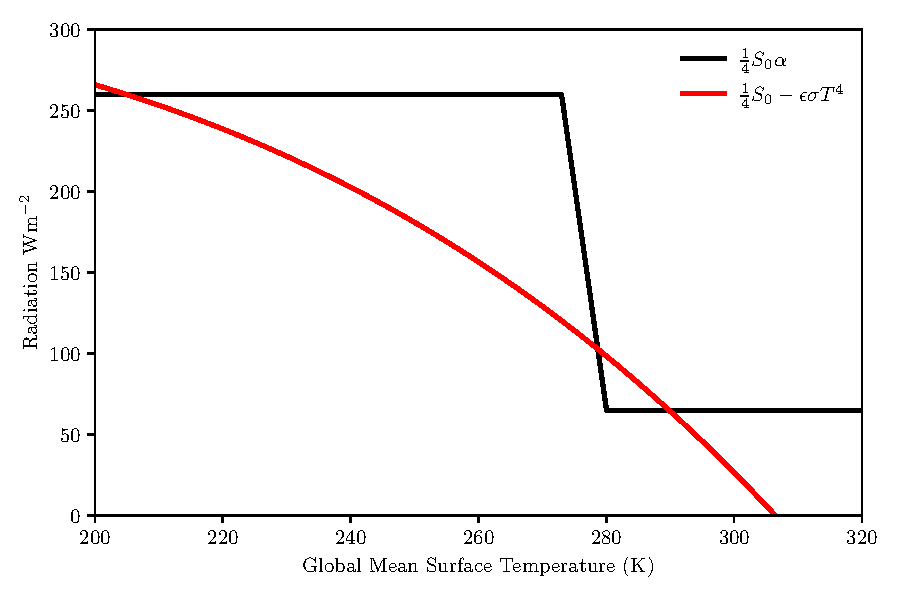
\includegraphics[width=\textwidth,keepaspectratio]{snowball}
  \caption[Snowball Earth Energy Balance]{The solutions to \cref{eq:energy_balance,eq:snowball_earth_albedo} are given by the intersections of these curves.
    The solution at $T\approx\SI{210}{\kelvin}$ is the snowball
    state and the solution at $T\approx \SI{290}{\kelvin}$ is the present day state. The intermediate state can be shown to be unstable and as such is not physically observable. The parameters were
    chosen somewhat arbitrarily,  but give a good approximation to the present day state. The parameters are $\alpha_+ = 0.8,\alpha_-=0.2,\epsilon=0.65,T_0 = \SI{280}{\kelvin},S_0 = \SI{1300}{\watt\per\meter\squared}$
    and $\sigma = \SI{5.67e-8}{\watt\per\meter\squared\per\kelvin\tothe{4}}$.}
  \label{fig:energy_balance_solution}
\end{figure}

This snowball state was predicted without empirical evidence, however decades after it was postulated evidence arose for its existence \parencite{Kirschvink1992,Hoffman2002}.
This state appears to have existed in the Neoproterozoic around \SI{650}{\mega\year\beforepresent}.
There is evidence for glaciers near the equator during this time. It is not clear
if the Earth was totally covered in ice, or if there was a think equatorial ocean, leading to a `slushball' Earth, rather than a `Hard Snowball' \parencite{Pierrehumbert2005,Pierrehumbert2011}.

\subsubsection{Dansgaard-Oeschger Events}
Less dramatic warm/cold transitions exist within the Earth system. During the Quaternary period, the Earth existed in interglacial and glacial states \parencite{Lisiecki2005}. Within the last glacial period,
around \SIrange{100}{10}{\kilo\year\beforepresent}, there were rapid transitions between cool stadial and warmer interstadial states \parencite{Oeschger1984,Dansgaard1993}. These transitions were discovered
in ice cores from Greenland, and represent rapid (on the timescale of 10 years) warming, some of which are up to \SI{16.5}{\kelvin} \parencite{Kindler2014}. However the relaxation period
back to the stadial state is longer, occurring on centennial timescales. A record of the Dansgaard-Oeschger events is plotted in \cref{fig:ngrip}. There is evidence that these Dansgaard-Oeschger events
had a global impact as ice core records show synchronous changes in Antarctica \parencite{Buizert2015}.

\begin{figure}
  \centering
  \includegraphics[width=\textwidth,keepaspectratio]{ngrip}
  \caption[NGRIP record of Dansgaard Oeschger events]{A record of $\delta \ce{^{18}O}$ from the NGRIP ice core from Greenland \parencite{NGRIP2004} over the last $100,000$ years.
    Higher values correspond to warmer temperatures. The clear spikes in this record are Dansgaard-Oeschger events. Note the rapid warming and slower cooling.}
  \label{fig:ngrip}
\end{figure}

There is no consensus on the mechanisms of the Dansgaard-Oeschger events, but they are generally believed to be caused by the subtle interplay of atmospheric, sea ice and AMOC dynamics
\parencite{Vettoretti2022,Boers2018,Riechers2023arxiv}. There is ongoing debate about the nature of the transition observed in Dansgaard Oeschger events, with different researchers arguing
that Dansgaard Oeschger events are driven stochastically \parencite{Ditlevsen2010,Ditlevsen1999} or deterministically \parencite{Boers2018a}.

\subsubsection{Green Sahara}
In the more recent past, a different sort of abrupt shift happened involving the biosphere. During the early part of the Holocene there was a northward expansion of shrub and savannah ecosystems
into what was the Sahara desert, as revealed in the pollen record \parencite{Hoelzmann1998,Hely2014}. This is therefore a `greening' of the Sahara. It was a time of enhanced rainfall \parencite{Tierney2017}
and is termed the African Humid Period.

The African Humid Period came to an end between \SIrange{6000}{4000}{\year\beforepresent}. Different reconstructions \parencite{Shanahan2015,Kropelin2008} disagree on how abrupt the transition
was, which may relate to the different regions involved in the reconstruction. An explanation for this 
involves a biogeophysical feedback proposed by Jule Charney \parencite{Charney1975,Charney1975a}. The mechanism is that vegetated ground has a lower
albedo than non-vegetated ground, so decreasing the vegetation increases the albedo, leading to decrease in net incoming radiation and a radiative cooling of the atmosphere, and so the air sinks by adiabatic compression
which inhibits convection and thus rainfall. This decrease in rainfall would then cause a further vegetation decrease.

Some climate models \parencite{Renssen2006} found that the transition was not abrupt. However, more recent work \parencite{Hopcroft2021} using a model that was tuned with mid-Holocene data was able to simulate an abrupt transition.

\section{Summary}
This chapter has given an introduction to climate tipping points as well as the coupled climate-carbon system. I have described some of the main processes at work
which govern the climate-carbon system and examined some climate tipping points. In the next chapter, the mathematical theory that underlies tipping points will be explored.
In addition, I will provide an introduction to early warning signals for tipping points.